\documentclass[autodetect-engine,dvipdfmx-if-dvi,ja=standard,everyparhook=compat]{bxjsarticle}

\usepackage{graphicx}        % 図を表示するのに必要
\usepackage{color}           % jpgなどを表示するのに必要
\usepackage{amsmath,amssymb} % 数学記号を出すのに必要
\usepackage{type1cm}         % fontsizeのエラー回避
\usepackage{here}            % 図の強制配置
\usepackage{url}             % URLをいい感じにしてくれる
\usepackage{subfigure}       % 図をまとめて表示
\usepackage{pdfpages}        % PDFの連結
\usepackage{setspace}
\usepackage{cases}
\usepackage{fancyhdr}
\usepackage{wrapfig}% 図の回り込み


% 余白の設定
% \setlength{\textheight}{\paperheight}   % 紙面縦幅を本文領域にする(BOTTOM=-TOP)
% \setlength{\topmargin}{-15.4truemm}     % 上の余白を10mm(=1inch-15.4mm)に
% \addtolength{\topmargin}{-\headheight}  %
% \addtolength{\topmargin}{-\headsep}     % ヘッダの分だけ本文領域を移動させる
% \addtolength{\textheight}{-20truemm}    % 下の余白も10mm
% \setlength{\textwidth}{\paperwidth}     % 紙面横幅を本文領域にする(RIGHT=-LEFT)
% \setlength{\oddsidemargin}{-5.4truemm}  % 奇数ページの左の余白を20mm(=1inch-5.4mm)に
% \setlength{\evensidemargin}{-5.4truemm} % 偶数数ページの左の余白を20mm(=1inch-5.4mm)に
% \addtolength{\textwidth}{-40truemm}     % 右の余白も20mm

% タイトル
\title{タイトル}

% ヘッダとフッタの設定
% \lhead{電気電子情報工学実験}
% \chead{}
% \rhead{20315784 佐藤凌雅}
% \lfoot{}
% \cfoot{\thepage} % ページ数
% \rfoot{}

\parindent = 0pt  % 行頭の字下げをしない
\setstretch{1.0}  % 行間

% キャプションの英語化
\renewcommand{\figurename}{Fig.}
\renewcommand{\tablename}{Table}

% 各章,節などタイトルの大きさを変更
% \titleformat*{\section}{\Huge\bfseries}
% \titleformat*{\subsection}{\Large\bfseries}

% 式の番号を(senction_num.num)のようにする
% \makeatletter
% \@addtoreset{equation}{chapter}
% \def\theequation{\thechapter.\arabic{equation}}
% \makeatother

% 呼び出したページのページ番号を消す
\newcommand{\deletePageNum}{
    \thispagestyle{empty}
    \clearpage
    \addtocounter{page}{-1}
}

% urlのフォントを直す
\renewcommand\UrlFont{\rmfamily}


\begin{document}
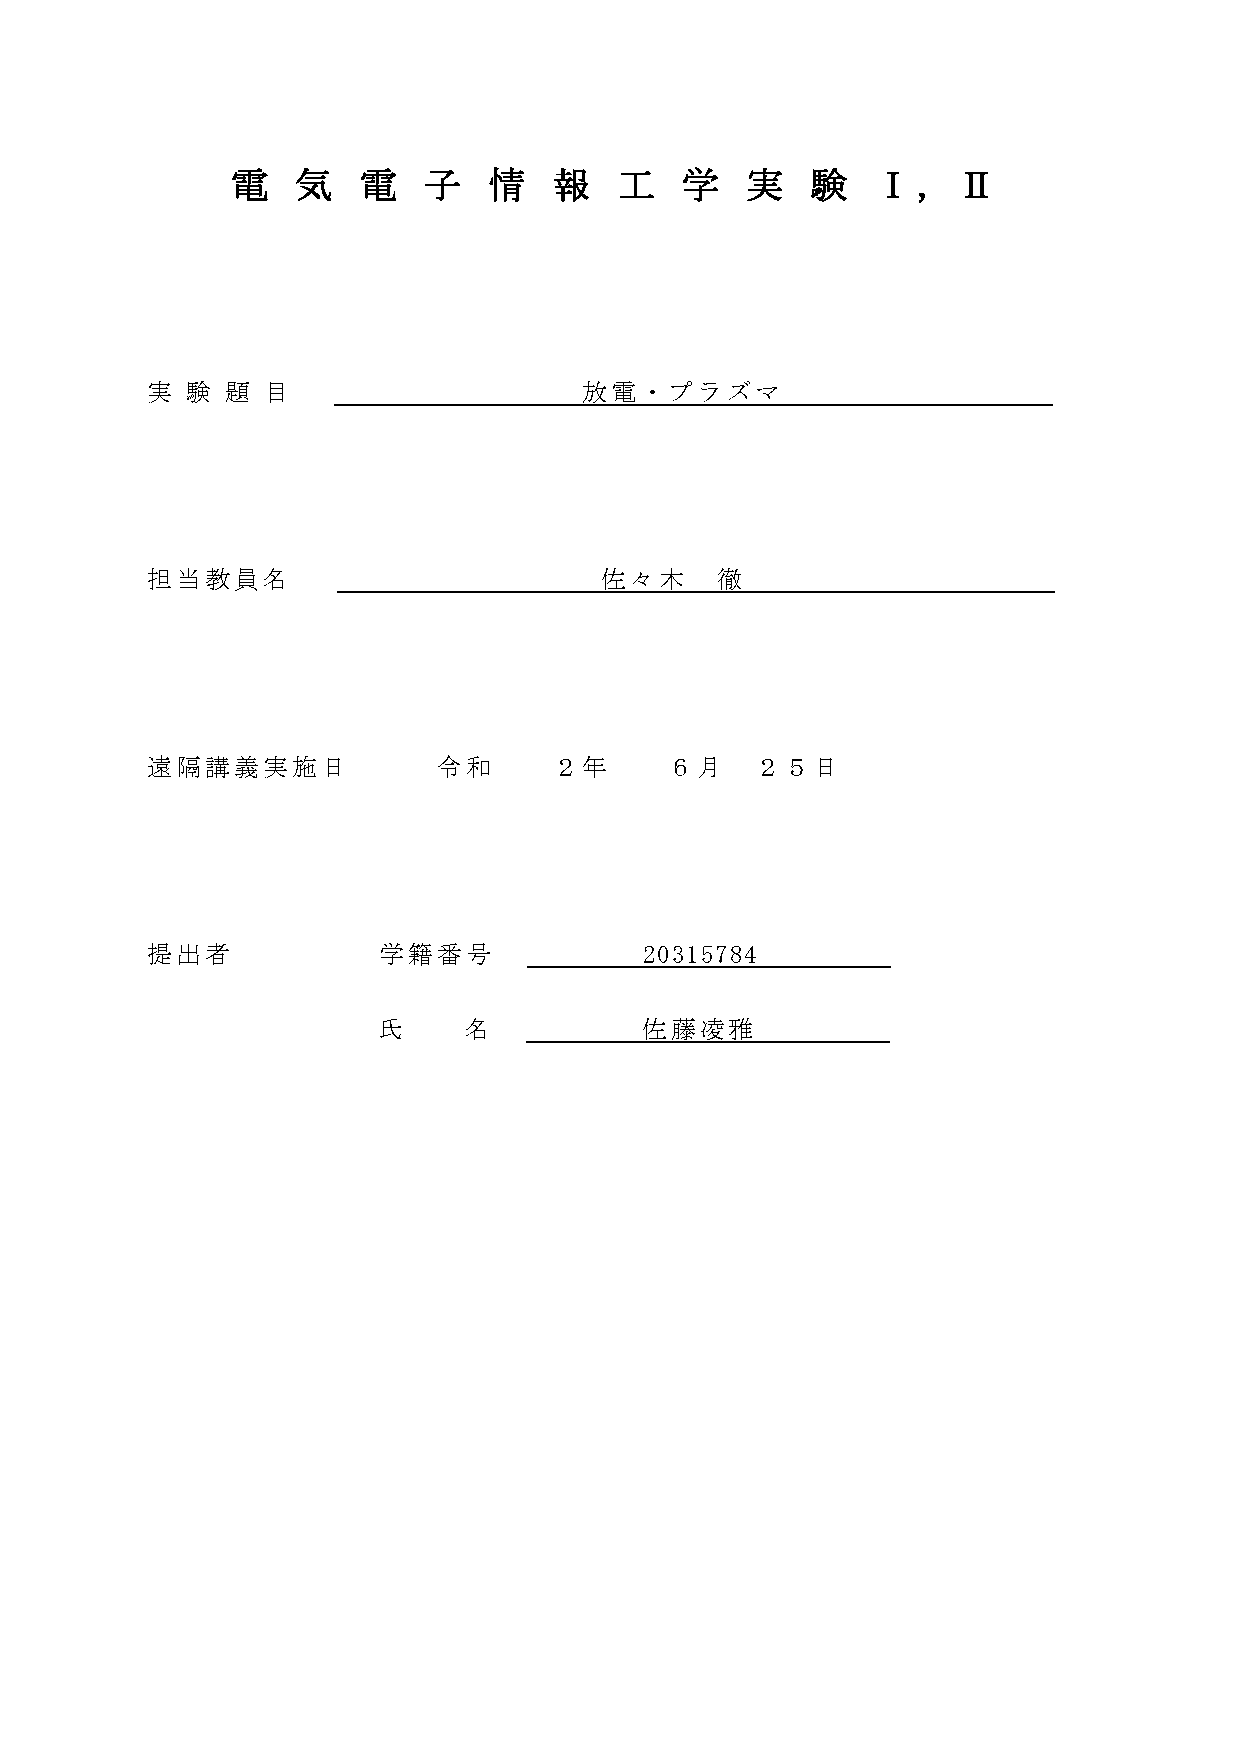
\includepdf[pages=-]{./setting/cover.pdf}
\fontsize{11.041pt}{16.562pt}\selectfont

\section{課題}
\subsection{写真と電圧電流特性からこの放電は何放電に対応するのかをこれまでの説明をもとに考察せよ.}
 0.5mA付近で大きな電圧の変化が見られるため,前期グロー放電であると考察する.

\newpage
\subsection{パッシェンの法則}
\subsubsection{パッシェンの法則を導出せよ}
\begin{eqnarray}
    \frac{\alpha}{P} &=& A \exp \left(-\dfrac{B}{\dfrac{E}{P}}\right) \nonumber\\
    \frac{\alpha}{P} &=& A \exp \left(-\dfrac{BP}{E}\right) \nonumber
\end{eqnarray}

 $E = \frac{V}{d}$を代入して
\begin{eqnarray}
    \frac{\alpha}{P} &=& A \exp \left(-\dfrac{BPd}{V}\right) \nonumber\\
    \frac{\alpha}{PA} &=& \exp \left(-\dfrac{BPd}{V}\right) \nonumber\\
    \ln\left(\dfrac{\alpha}{PA}\right) &=& -\dfrac{BPd}{V} \nonumber
\end{eqnarray}

 $V$について解くと
\begin{eqnarray}
    V_B &=& -\dfrac{BPd}{\ln\left(\dfrac{\alpha}{PA}\right)} \nonumber\\
        &=& -\dfrac{BPd}{\ln(\alpha) - \ln(P) - \ln(A)} \nonumber\\
        &=& \dfrac{BPd}{-\ln(\alpha) + \ln(P) + \ln(A)} \nonumber\\
        &=& \dfrac{BPd}{-\ln(\alpha) + \ln(P) + \ln(A) + \ln(d) - \ln(d)} \nonumber
\end{eqnarray}

 ここで,$K_0 = \ln(A) - \ln(\alpha)  - \ln(d)$とおくと,
\begin{eqnarray}
    V_B &=& \dfrac{BPd}{K_0 + \ln(P) + \ln(d)} \nonumber\\
        &=& \dfrac{BPd}{K_0 + \ln(Pd)} \nonumber
\end{eqnarray}

 なお,$K_0$は
\begin{eqnarray}
    K_0 &=& \ln(A) - \ln(\alpha)  - \ln(d) \nonumber\\
        &=& \ln \left(\frac{A}{\alpha d}\right) \nonumber\\
        &=& \ln \left(\frac{A}{\ln \left( \exp \left(\alpha d\right)\right)}\right) \nonumber\\
        &=& \ln \left(\frac{A}{\ln \left(1 + \exp \left(\alpha d\right) - 1\right)}\right) \nonumber
\end{eqnarray}

 $\gamma\left( \exp\left(\alpha d\right) -1 \right) = 1$より$\gamma = \left( \exp\left(\alpha d\right) -1 \right)^{-1}$に留意して
\begin{eqnarray}
    K_0 &=& \ln \left(\frac{A}{\ln \left(1 + \gamma^{-1} \right)}\right) \nonumber\\
        &=& \ln \left(A\right) - \ln \left(\ln \left(1 + \dfrac{1}{\gamma} \right)\right) \nonumber
\end{eqnarray}

\subsubsection{火花電圧$V_B$を最小とする$Pd$積とその時の火花電圧$V_{Bmin}$を求めよ}
 $V_B$が最小となるのは$\frac{dV_B}{d(Pd)} = 0$の時であるから,
\begin{eqnarray}
    \frac{dV_B}{d(Pd)} &=& \frac{d}{d(Pd)} \left(\dfrac{BPd}{K_0 + \ln(Pd)}\right) \nonumber\\
    &=& \dfrac{B \cdot (K_0 + \ln(Pd)) - BPd \cdot 1/Pd}{(K_0 + \ln(Pd))^2} \nonumber\\
    &=& \dfrac{B \cdot (K_0 + \ln(Pd) - 1)}{(K_0 + \ln(Pd))^2} \nonumber\\
\end{eqnarray}

$\frac{dV_B}{d(Pd)} = 0$の時は,分子が0の時なので,$B \cdot (K_0 + \ln(Pd) - 1) = 0$を解くと
\begin{eqnarray}
    B \cdot (K_0 + \ln(Pd) - 1) = 0 \nonumber \\
    \ln(Pd) = 1 - K_0 \nonumber \\
    Pd = \exp(1 - K_0) \nonumber
\end{eqnarray}

$P_d = \exp(1 - K_0)$を$V_B$に代入すると,
\begin{eqnarray}
    V_{Bmin} &=& \dfrac{BPd}{K_0 + \ln(Pd)} \nonumber \\
                    &=& \dfrac{B \exp(1 - K_0)}{K_0 + \ln (\exp(1 - K_0))} \nonumber \\
                    &=& \dfrac{B \exp(1 - K_0)}{K_0 + 1 - K_0} \nonumber \\
                    &=& B \exp(1 - K_0) \nonumber
\end{eqnarray}

\subsubsection{空気の場合の火花電圧-pd積のグラフを作成せよ.なお,A=15[cm$^{-1}$Torr$^{-1}$],B=365[Vcm$^{-1}$Torr$^{-1}$],$\gamma$=0.02とし,縦軸を$V_B$,横軸pd積は[Pa m]の単位系で記述すること.}
 A=15[cm$^{-1}$Torr$^{-1}$]=11.25[m$^{-1}$Pa$^{-1}$]\\
 B=365[Vcm$^{-1}$Torr$^{-1}$]=273.8[Vm$^{-1}$Pa$^{-1}$]より,$K_0$=1.051となるので,
\begin{eqnarray}
    V_B = \frac{273.8Pd}{1.051+\ln(Pd)}
\end{eqnarray}
となる.\\
これをグラフで表すとFig.\ref{fig:PaschenCurve}に示すようになる.
\begin{figure}[H]
    \centering
    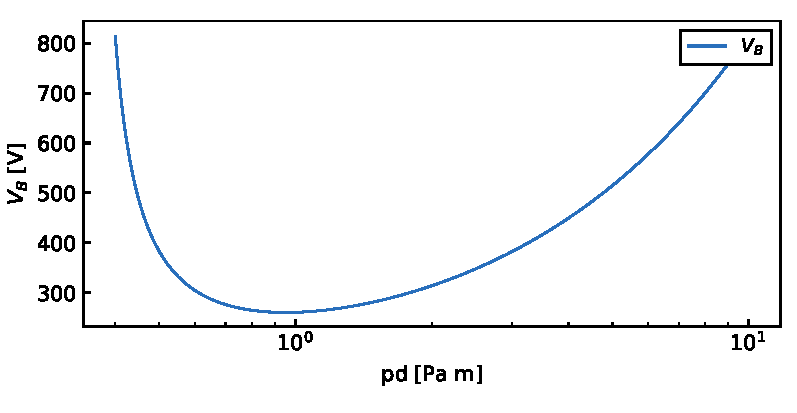
\includegraphics[width=11cm]{./fig/PaschenCurve.pdf}
    \caption{Paschen Curve}
    \label{fig:PaschenCurve}
\end{figure}

\newpage
\subsection{電子温度と電子密度を求める}
\subsubsection{プローブ電圧$V_p$-プローブ電流$I_p$特性のグラフを作る}
 作成したグラフをFig.\ref{fig:Vp-Ip}に示す.
\begin{figure}[H]
    \centering
    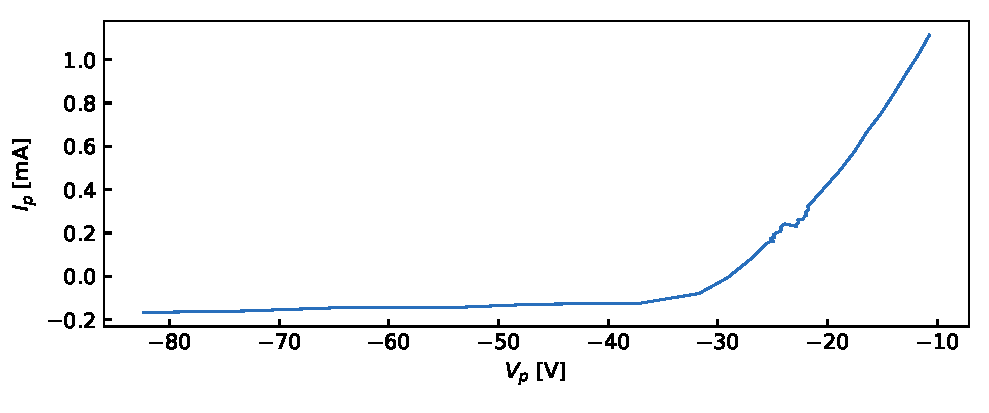
\includegraphics[width=11cm]{./fig/3_1.pdf}
    \caption{Graph of $V_p$-$I_p$ characteristics}
    \label{fig:Vp-Ip}
\end{figure}

\subsubsection{作ったプローブ電圧$V_p$-プローブ電流$I_p$特性からイオン飽和電流を求める}
 イオン飽和領域の傾きが緩やかな領域を延長し,y軸との交点がイオン飽和電流$I_{is}$となる.直線はイオン飽和領域の6点から最小二乗法を用いて引いた.作成したグラフをFig.\label{fig:Vp-Ip-iis}に示す.最小二乗法によって求めた直線の切片から,イオン飽和電流$I_{is}$は0.087[mA]であることがわかった.
\begin{figure}[H]
    \centering
    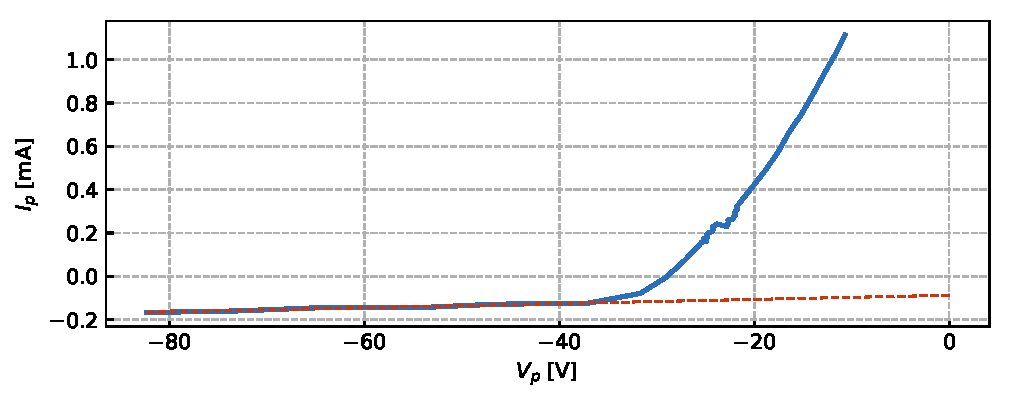
\includegraphics[width=11cm]{./fig/3_2.pdf}
    \caption{Graph of $V_p$-$I_p$ characteristics}
    \label{fig:Vp-Ip-iis}
\end{figure}

\subsubsection{求めたイオン飽和電流を使って,プローブ電圧$V_p$-プローブ電流$I_e$特性を作る}
 プローブ電流$I_p$,電子電流$I_e$,イオン電流$I_i$の間には以下の関係が成立する.
\begin{eqnarray}
    I_p = I_e + I_i
\end{eqnarray}
 このとき,イオン飽和電流$I_{is}$がイオン電流$I_i$とおおよそ等しいと仮定すると
\begin{eqnarray}
    I_p = I_e + I_{is}\nonumber\\
    I_e = I_p - I_{is}
\end{eqnarray}
 以上を踏まえて,プローブ電圧$V_p$-プローブ電流$I_e$特性を描くと,Fig.\ref{fig:Vp-Ie}が得られる
\begin{figure}[H]
    \centering
    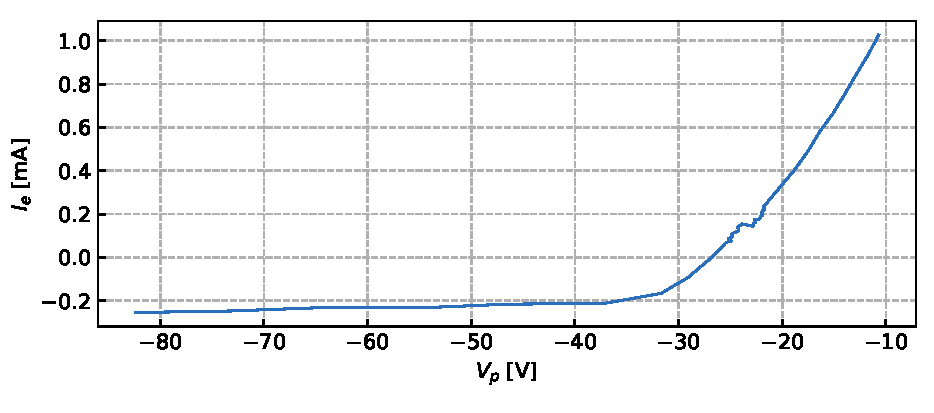
\includegraphics[width=11cm]{./fig/3_3.pdf}
    \caption{Graph of $V_p$-$I_e$ characteristics}
    \label{fig:Vp-Ie}
\end{figure}

\subsubsection{3.で作った特性から工夫をして,電子温度を出す}
$\frac{d}{dV_p} \ln\left(I_e(V)\right) = \frac{e}{k_B T_e}$より,電子温度$T_e$は以下で求められる.
\begin{eqnarray}
    T_e = \frac{e}{k_B}\cdot\left(\frac{d}{dV_p} \ln\left(I_e(V)\right)\right)^{-1}
\end{eqnarray}
 ここで,$\frac{d}{dV_p} \ln\left(I_e(V)\right)$を求めるために,Fig.$V_p$-$\ln(I_e)$特性を描く.
\begin{figure}[H]
    \centering
    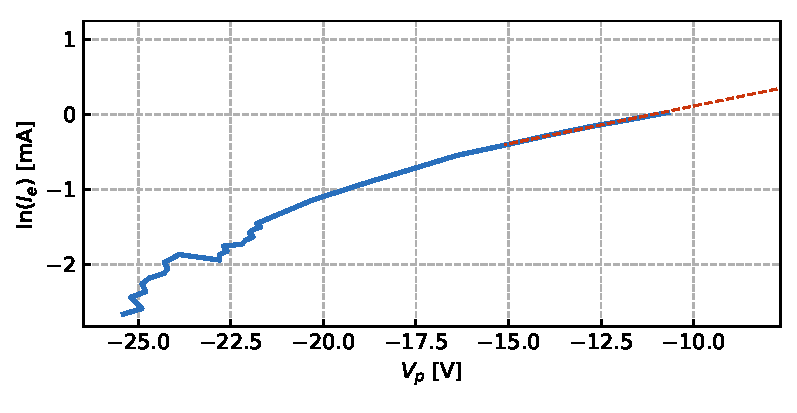
\includegraphics[width=11cm]{./fig/3_4.pdf}
    \caption{Graph of $V_p$-$\ln(I_e)$ characteristics}
    \label{fig:Vp-lnIe}
\end{figure}
 このグラフにおいて,橙色の線は$V_f$近傍の接線であり,この傾きが$\frac{d}{dV_p} \ln\left(I_e(V)\right)$となる.$\frac{d}{dV_p} \ln\left(I_e(V)\right)$は0.10であることがわかった.よって,電子温度$T_e$は$k_B=1.38\times10^{-23}$J/K,$e=1.6\times10^{-19}$であることに留意して
\begin{eqnarray}
    T_e = \frac{e}{k_B}\cdot\left(\frac{d}{dV_p} \ln\left(I_e(V)\right)\right)^{-1} = \frac{1.6\times10^{-19}}{1.38\times10^{-23}}\cdot(0.1)^{-1} = 115942
\end{eqnarray}


\subsubsection{4.で求めた電子温度を利用して,電子密度を求める.なお,プローブ表面積$S_p$は$5 \times 10^{-5}$m$^2$とする.また,電子密度の単位を示すこと.}
\begin{eqnarray}
    I_{is} &=& \exp\left(-\frac{1}{2}\right)en_eS_p\sqrt{\frac{k_BT_e}{M_i}}\nonumber\\
    n_e &=& I_{is}\left(\exp\left(-\frac{1}{2}\right)eS_p\sqrt{\frac{k_BT_e}{M_i}}\right)^{-1}\nonumber\\
    &=& 8.7\times10^{-5}\left(\exp\left(-\frac{1}{2}\right)\cdot 1.6\times10^{-19} \cdot 5 \times 10^{-5} \cdot \sqrt{\frac{1.38\times10^{-23}\cdot115942}{40\times1.6\times10^{-27}}}\right)^{-1}\nonumber\\
    &=&3.58\times10^{14}[\mbox{m}^{-3}]
\end{eqnarray}

% % 実験の目的,手段,結果,結論を簡潔にまとめ示すこと.(250字程度)
% \section{概要 Abstract}


% % テキストに書かれている目的等を参考に,各自どの点に注目して実験したのかを明確に示すこと.(300字程度)
% \section{目的 Purpose}


% % 各自の実験目的に必要な理論的な背景を示すこと.必要ならば,参考文献リストより文献番号を引用すること.(レポート用紙1枚程度)
% \section{理論的背景 Theory}


% % 実験手段,測定系の概要,測定装置の名称・型番等を書くこと.また,装置の精度・仕様等の情報もできる限り示すこと.(レポート用紙2枚程度)
% \section{実験方法 Experiment}


% % 各自の実験目的に沿った結果を簡潔にまとめること.その他の試行錯誤的実験データは Appendix にまとめる.枚数は各教員の指示に従ってください.(レポート用紙の枚数は教員の指示に従う)
% \section{実験結果 Results}

% % 各自の目的と照らし合わせ,測定結果の妥当性や数値計算結果との整合性などについて考察する.実験結果とサブテキスト/参考書の図式とを比較し議論すること.課題が与えられているテーマに関してはそれについても考察すること.(レポート用紙2枚程度)
% \section{考察 Discussion}

% % 君自身が実験を通じて(実験の方法,まとめ方などで)工夫した点をまとめる.(100字程度 )
% \section{工夫した点}

% 実験結果の羅列ではなく,考察した結果をまとめること.(250字程度)
% \section{まとめ Conclusion}

% レポートで引用した参考文献のリストを付ける.
% \begin{thebibliography}{9}
%     \bibitem{denkikigairon} 深尾正 (2015). 電気機器概論. 実教出版株式会社.
% \end{thebibliography}


% % 周辺の関連調査事項,作成プログラムリスト,試行錯誤的実験データ
% \appendix
% \section{Appendix}

\end{document}
